\section{Illustrative example%: The impossibility of direct reverse engineering generated code
	}
\label{sec:motivation}

We consider a producer-consumer example developed using component-based engineering.
Fig. \ref{fig:cbseexample} (left) shows the component-based model of the example.
The \ttt{p} producer produces data items and sends to a first-in first-out passive communication channel instance \ttt{fifo}.
The latter stores data in order for the consumer to pull it.
The class diagram of \ttt{FIFO} is explored in Fig. \ref{fig:cbseexample} (right).
FIFO persists data items in a sized queue attribute, namely, \ttt{queue}.
The latter is associated with the number of currently stored items (\ttt{numberOfItems}), the capacity (\ttt{MAX\_SIZE}), and other attributes and operations used for validating incoming items and the status of the queue.

The producer's port with \ttt{IPush} as its required interface is connected to the port of FIFO with \ttt{IPush} as its provided interface so that the producer and FIFO can interact with each other through their respective port.
Because FIFO provides two interfaces, it implements these.

The behavior of \ttt{FIFO} is described by using a UML State Machine as in Fig. \ref{fig:fifostatemachine}.
The machine activates the \ttt{Idle} state as initial state.
The latter waits for an item to come to the \ttt{fifo} component (through the \ttt{pPush} port, for instance).
The item is then checked for its validity by using a \ttt{choice} pseudo state.
The \ttt{DataQueuing} state verifies the status of the queue to decide to either add the item to the queue or discard it.  


\begin{figure}
	\centering
	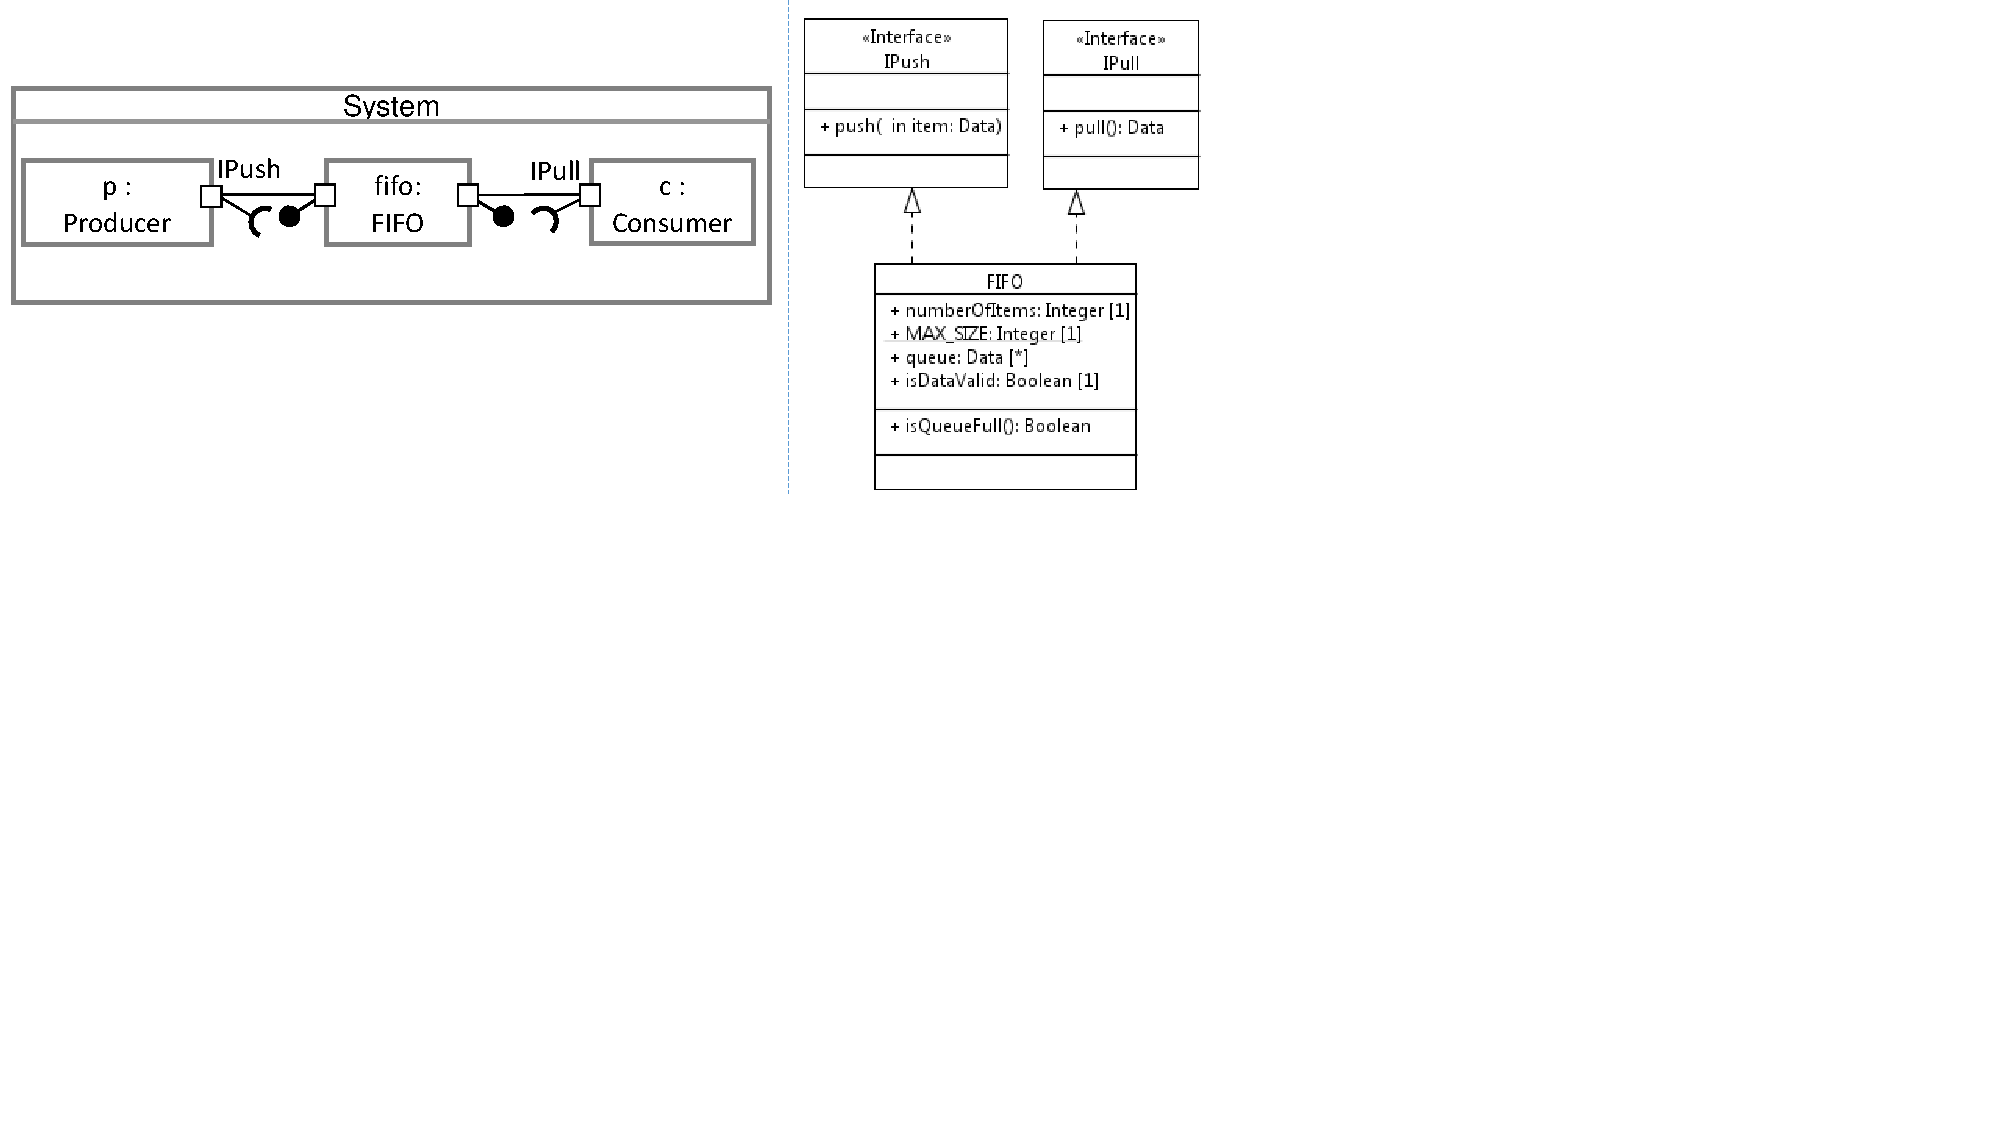
\includegraphics[clip, trim=0cm 14.9cm 14.9cm 0cm, width=\columnwidth]{figures/cbseexample.pdf}
	\caption{Architecture of System (left) and Class diagram of FIFO (right)} 
	\label{fig:cbseexample}
\end{figure}


\begin{figure}
	\centering
	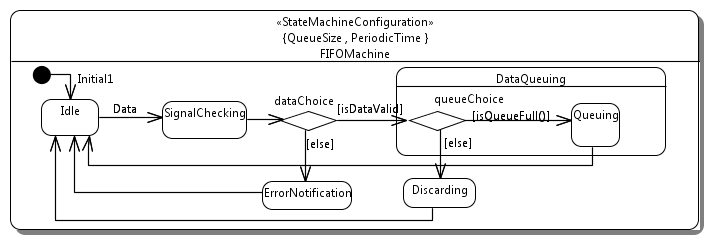
\includegraphics[clip, trim=0.2cm 0cm 0cm 0.1cm, width=1.0\columnwidth]{figures/fifostatemachine.png}
	\caption{FIFO's UML State Machine} 
	\label{fig:fifostatemachine}
\end{figure}

In the next sections, this example will be used for illustrating how XSeparation works.


%Let's consider a collaboration scenario between software architects and programmers in developing an event-driven paradigm-based system \ttt{System}. 
Fig. \ref{fig:illustration} (a) and (b) show the current and evolved USM behaviors of \ttt{System}.
%The latter's behavior is described by using a USM as in Fig. \ref{fig:IllustrationExample1}.
%This USM is artificial, and is extracted and customized from the origin in \cite{shuang_formalizing}.
This USM consists of some simple, composite, and pseudo states such as \ttt{choice}, \ttt{entry point}, and \ttt{history}.

\begin{figure}
	\centering
	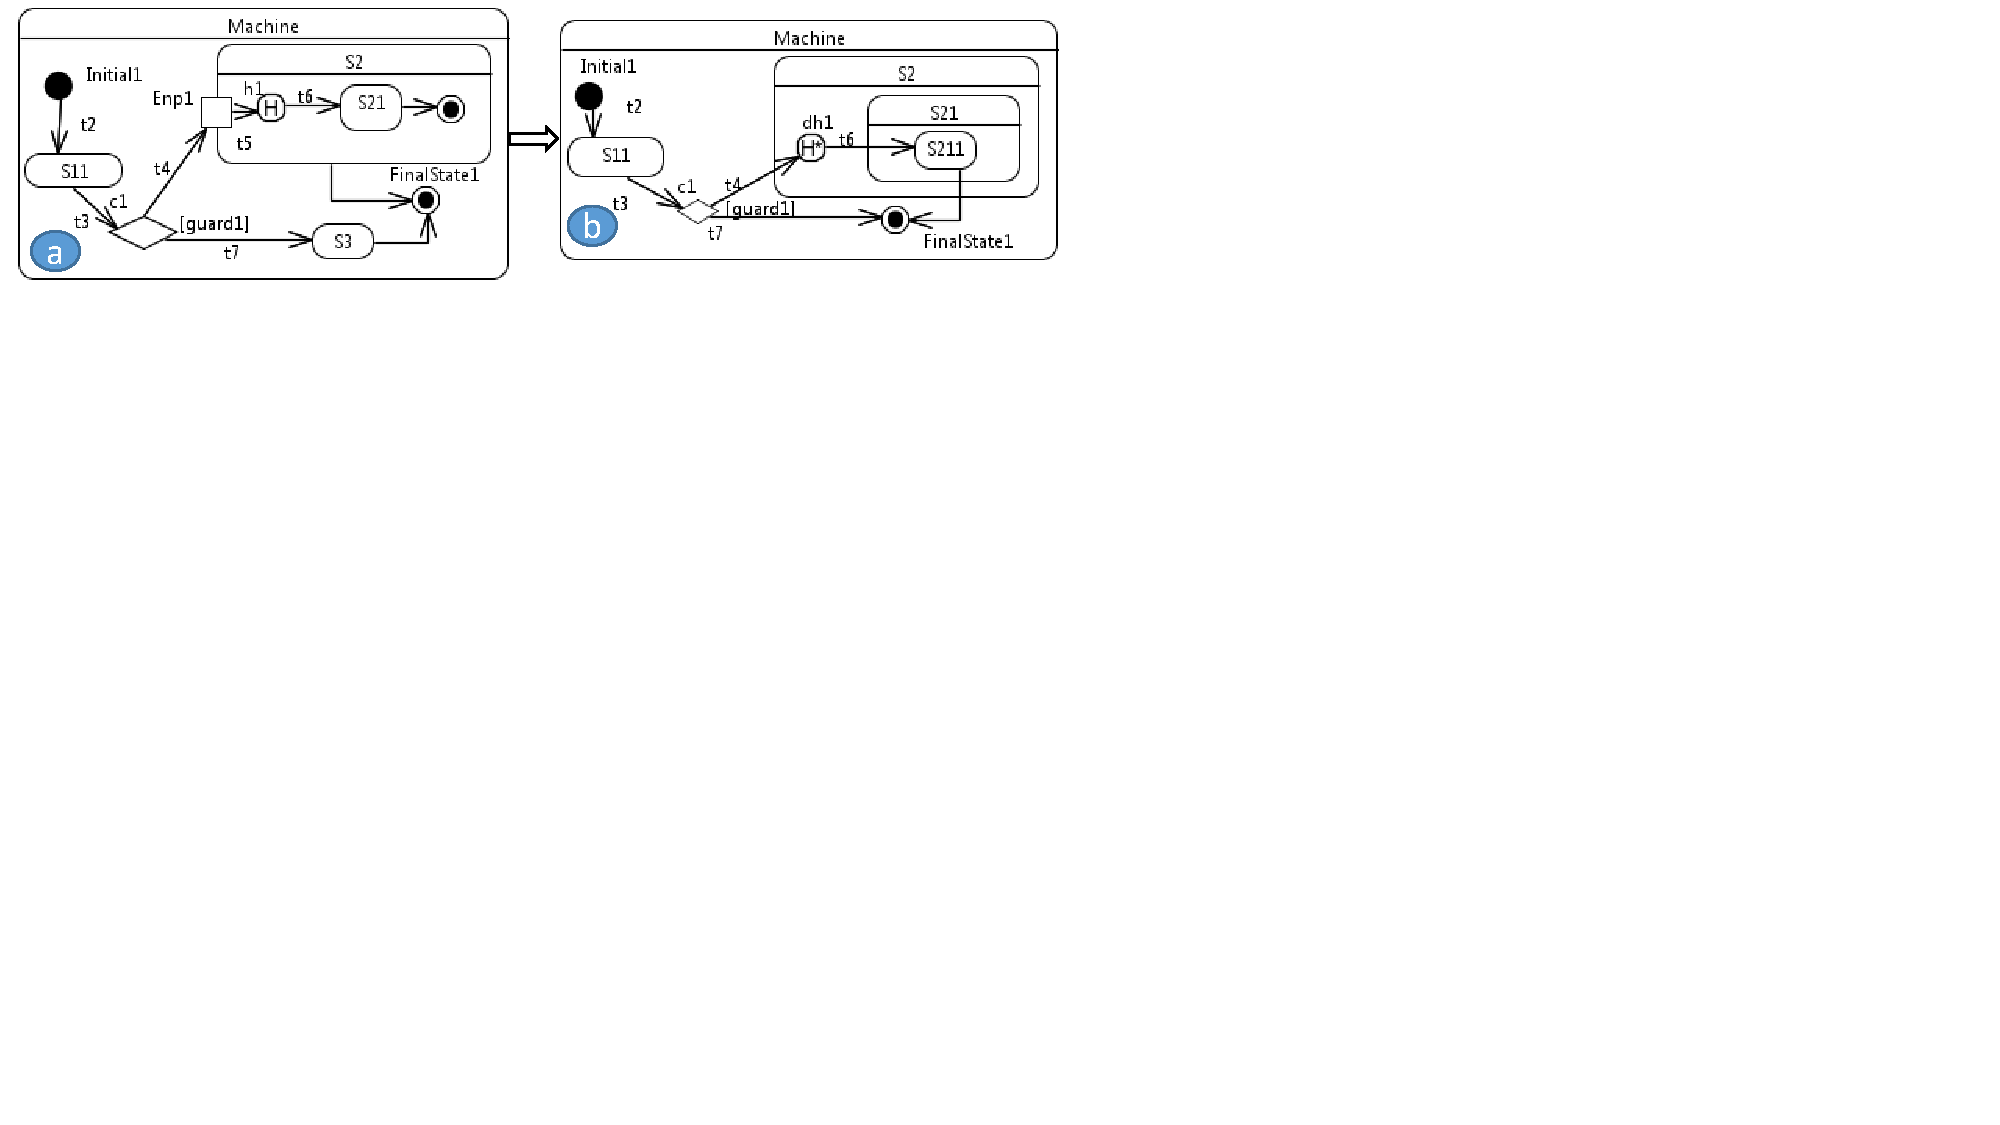
\includegraphics[clip, trim=0.2cm 14cm 15.8cm 0.1cm, width=1.0\columnwidth]{figures/illustration}
	\caption{A USM example (a) and its evolved version (b).} 
	\label{fig:illustration}
\end{figure}


\begin{comment}
\begin{figure}
	\centering
	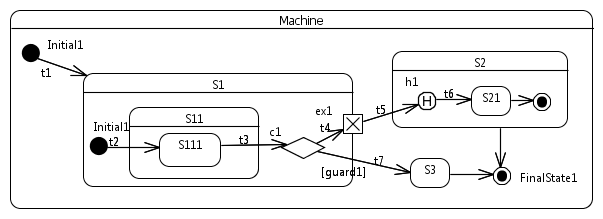
\includegraphics[clip, trim=0.2cm 0.2cm 0.2cm 0.2cm, width=1.0\columnwidth]{figures/IllustrationExample1.png}
	\caption{A USM example} 
	\label{fig:IllustrationExample1}
\end{figure}

\begin{figure}
	\centering
	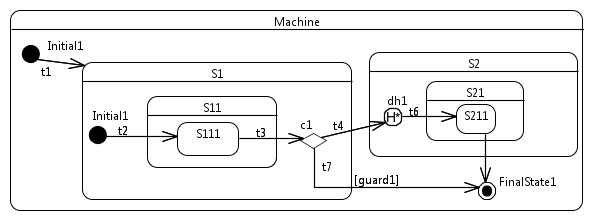
\includegraphics[clip, trim=0.2cm 0.2cm 0.1cm 0.2cm, width=1.0\columnwidth]{figures/IllustrationExample2.png}
	\caption{The evolved version of the USM shown in Fig. \ref{fig:IllustrationExample1}} 
	\label{fig:IllustrationExample2}
\end{figure}



\begin{figure}
	\centering
	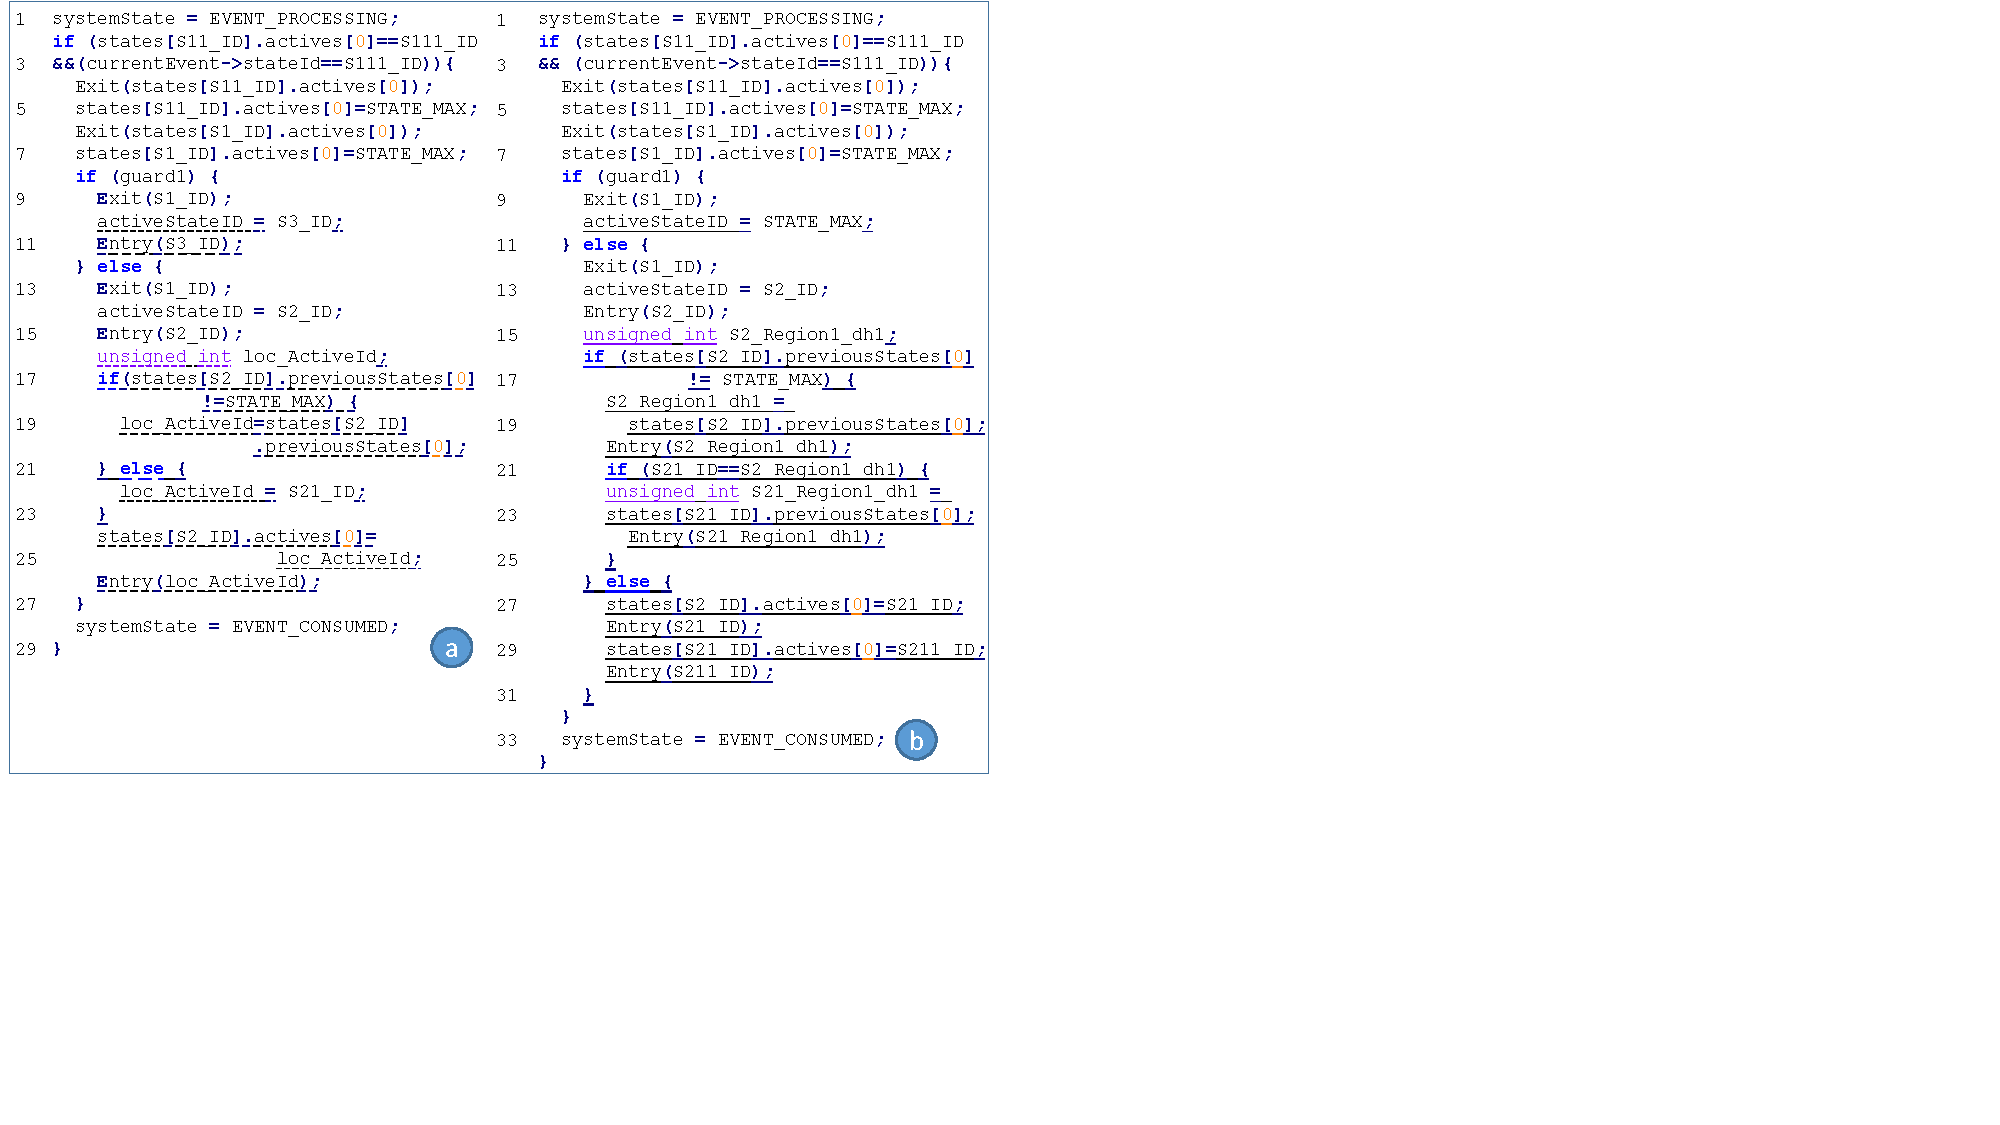
\includegraphics[clip, trim=0.15cm 5.9cm 17.1cm 0.0cm, width=1.04\columnwidth]{figures/highlight.pdf}
	\caption{Codes generated from the state machine example in Fig. \ref{fig:illustration} by using our tool (a) and Rhapsody (b), and their respective evolved versions. The \protect\dashuline{dashed underlined code} segment should evolve to the \protect\uline{simple underlined code}.} 
	\label{fig:generatedcode}
\end{figure}
\end{comment}





\begin{comment}
\begin{figure*}
	\centering
	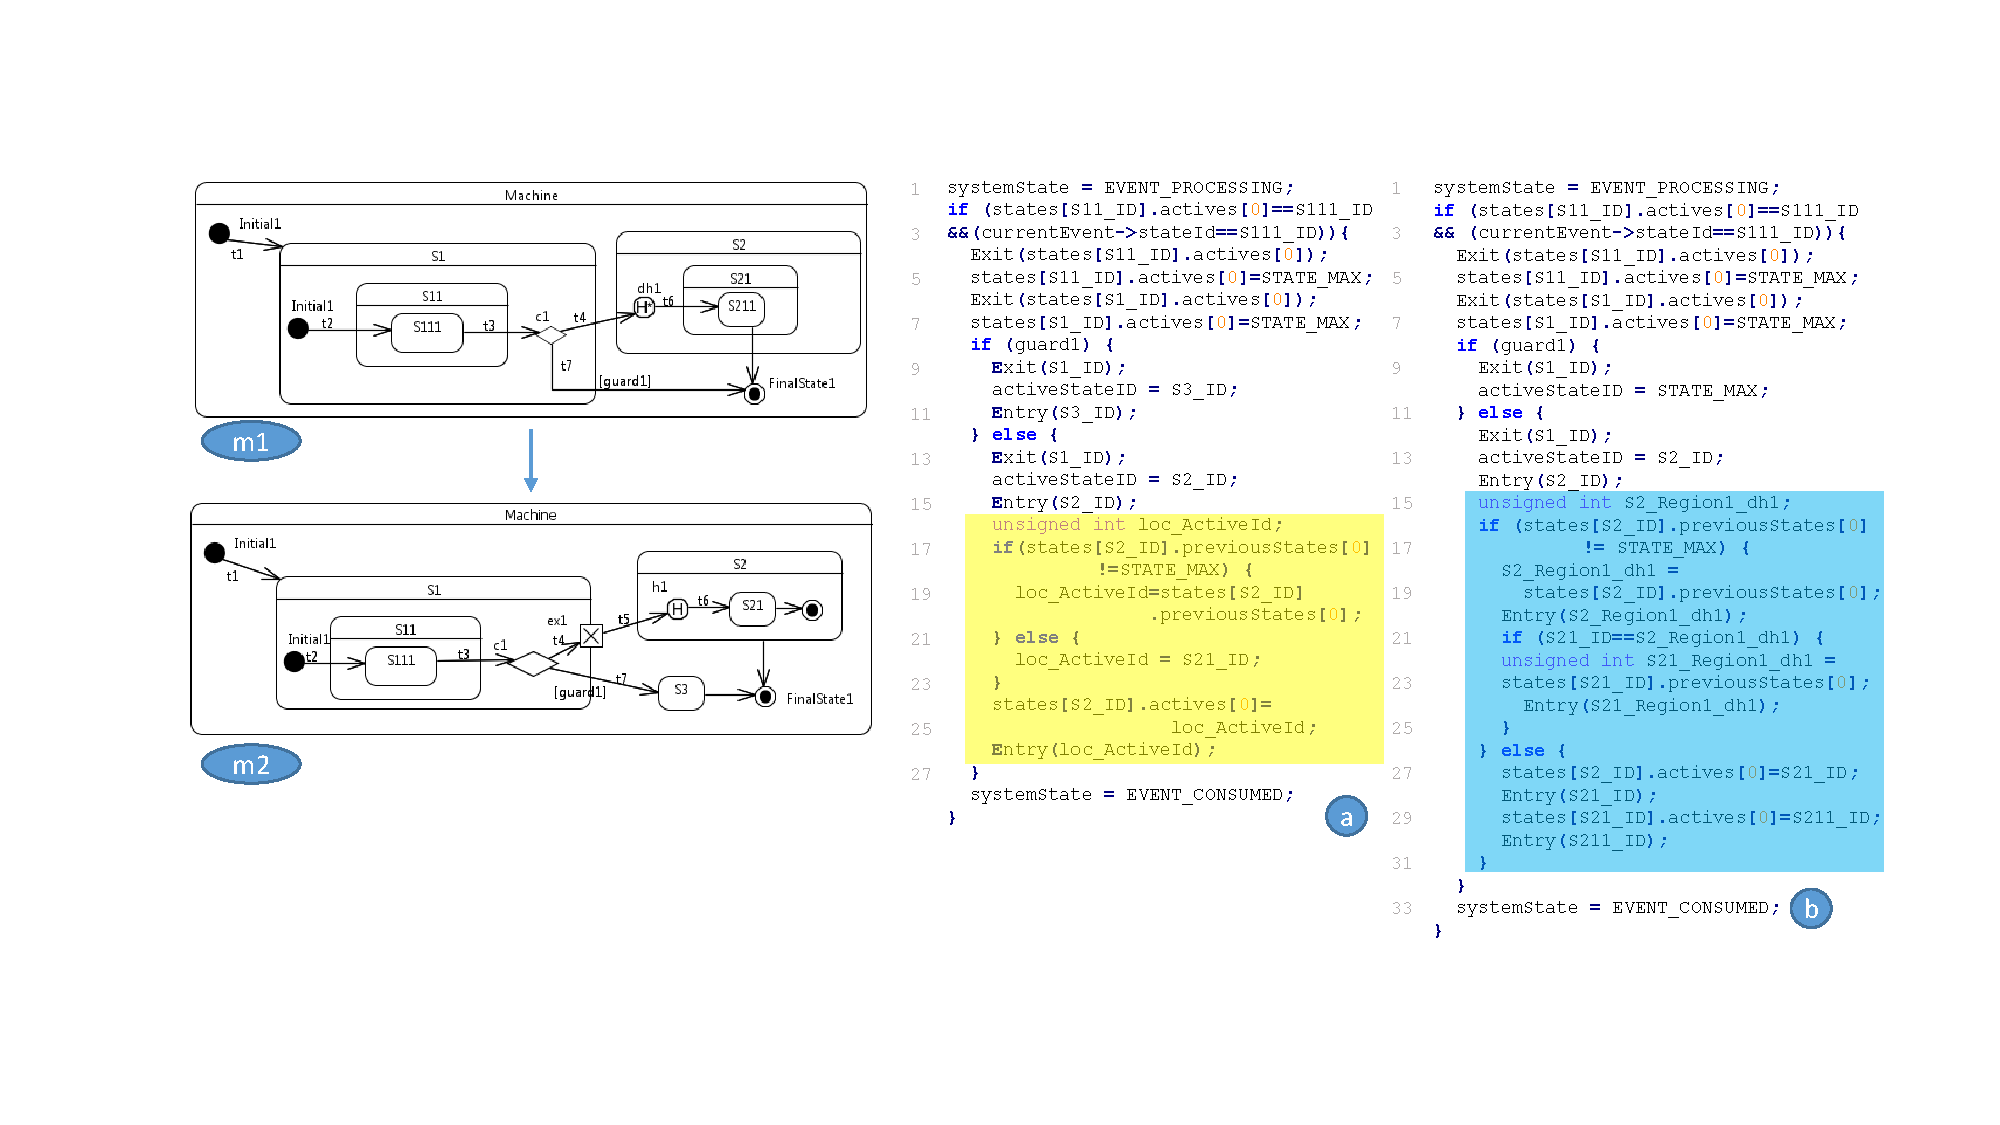
\includegraphics[clip, trim=3.2cm 3.2cm 2.0cm 2.2cm, width=1.0\textwidth]{figures/generatedcodebig2}
	\caption{The evolved version of the USM shown in Fig. \ref{fig:generatedcode}} 
	\label{fig:generatedcode}
\end{figure*}
\end{comment}

%Although many tools have the ability to generate code from USMs, 
Only a few tools such as IBM Rhapsody \cite{ibm_rhapsody}, Papyrus-RT \cite{possepapyrusrt} and ours are able to deal with this example because generating code for pseudo states such as \ttt{entry point} and \ttt{history} is not as simple as states.
Listing \ref{lst:generated1} shows the code segment generated for the transition outgoing from the state \ttt{S11} of the example in Fig. \ref{fig:illustration} (a). 
%and its evolved version by using our tool, respectively.

\begin{minipage}{0.95\columnwidth}
\lstinputlisting[language=C++, caption=Code generated from the state machine example in Fig. \ref{fig:illustration} (a), label=lst:generated1,frame=f]{code/generated1.cpp}
\end{minipage}



%In this scenario, we assume that, on one hand, programmers prefer to
%use the more familiar textual programming language. 
%On the other hand, software architects, working at higher levels
%of abstraction, tend to favor the use of models, and therefore
%prefer graphical languages for describing the high-level logic behavior by using modeling tools.

%In this scenario, we assume that, for some reasons, the USM should be evolved to the next version as in Fig. \ref{fig:IllustrationExample2}.


For simplification, we assume that no effects are associated with the transitions in the examples.
In Listing \ref{lst:generated1} (a), the segment checks whether the state \ttt{S11} is active (line 1).
If so, the exit actions of \ttt{S11} is executed (line 2).
The segment then evaluates \ttt{guard1} (lines 3 and 5) to dynamically select which transition outgoing from the choice \ttt{c1} should be taken into account.
If \ttt{guard1} is false, the entry action of \ttt{S2} (line 6) is called and the restoration of the previous active sub-state of \ttt{S2} (lines 7-14) is executed. 
Otherwise, \ttt{S3} is entered (line 6).

The code for the USM in Fig. \ref{fig:illustration} (b) differs from that of Fig. \ref{fig:illustration} (a) by the way the history of \ttt{S2} is restored.
Listing \ref{lst:generated2} shows how the deep restoration for the deep history pseudo state in Fig. \ref{fig:illustration} (b) in lines 5-16 if \ttt{guard1} is evaluated as false.
These lines actually read the previous active sub-state of not only \ttt{S2} (lines 7-8) but also \ttt{S21} (lines 10-11), and set these states as current active sub-states.

\begin{minipage}{0.95\columnwidth}
\lstinputlisting[language=C++, caption=Code generated from the example in Fig. \ref{fig:illustration} (b) differs from that of Fig. \ref{fig:illustration} (a), label=lst:generated2,frame=f]{code/generated2.cpp}
\end{minipage}

%It is worth noting that, 
The code generation patterns are not explicitly understandable for the programmers to capture the control flow of the USM. %associated with the code.
Hence, it is challenging to modify the topology of the USM at the code level. 
Even, if the programmers could understand and modify the code %following the used patterns, which require a very high discipline
, it is still very difficult for RTE tools to decipher and reflect the code changes to the model.
Furthermore, 
%code generation patterns produce different code looks.
%As a result, 
it is very hard, if not impossible, to find common rules to reconstruct the original state machine from the code. 
This is the reason why existing RTE tools such as Rhapshody 
%supporting round-trip engineering 
have no way to recover the modified code to the original USM.



Some approaches use interactive grammar interference \cite{walkinshaw2007reverse}, clustering \cite{hall2010superstate}, or static analysis \cite{DBLP:conf/kbse/AbadiF12} to produce state machine diagrams from legacy code.
However, the diagrams produced by these approaches usually contain too many states and are only used for system understanding and documentation. 

Consequently, to interfere the high-level logic behavior of the systems, the programmers must use the click-and-select mechanism of modeling tools, which do, as previously, not encourage programmers. 
Furthermore, it does not guarantee the seamless collaboration between the favored practices of programmers and software architects.  

In the next section, we show how RAOES can handle this collaboration problem.

